\setbeamercovered{invisible}
\begin{figure}
    \centering
    \resizebox{!}{.8\textheight}{
        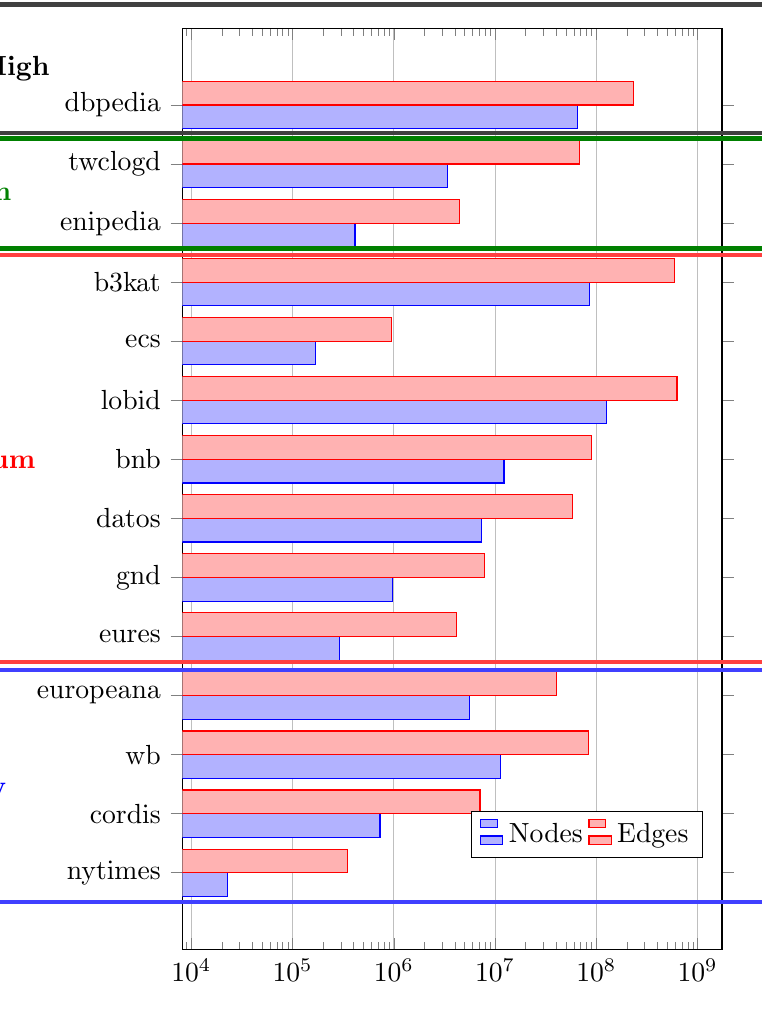
\begin{tikzpicture}
            \begin{axis}[
                    xbar=0pt,
                    y=.75cm,
                    symbolic y coords={nytimes,cordis,wb,europeana,eures,gnd,datos,bnb,lobid,ecs,b3kat,enipedia,twclogd,dbpedia},
                    bar width=0.3cm,
                    ytick=data,
                    xmode = log,
                    xmajorgrids = true,
                    legend style={at={(0.75,0.15)}, anchor=north,legend columns=-1},
                ]
                \addplot coordinates { (22662,nytimes) (729780,cordis) (11210832,wb) (5559452,europeana) (288862,eures) (962930,gnd) (7412312,datos) (12246306,bnb) (124691274,lobid) (167390,ecs) (85795956,b3kat) (413520,enipedia) (3398947,twclogd) (65042837,dbpedia) };
                \addplot coordinates { (345888,nytimes) (7101623,cordis) (84345613,wb) (40773834,europeana) (4146421,eures) (7940373,gnd) (58048932,datos) (89733453,bnb) (625941644,lobid) (955112,ecs) (592778746,b3kat) (4463566,enipedia) (67505792,twclogd) (233051608,dbpedia) };
                \legend{Nodes,Edges}
            \end{axis}

            \uncover<2->{
                %\draw[step=1cm,gray,ultra thick,overlay] (-20,-2) grid (20,12);
                %\draw[step=.1cm,blue,overlay] (-20,-2) grid (20,12);
                % very high
                \draw[black!75,ultra thick,overlay] (-13,12) rectangle (7.8,10.37) node[midway] {\textbf{\textcolor{black}{Very High}}};
                % high
                \draw[black!50!green,ultra thick,overlay] (-13,10.3) rectangle (7.8,8.9) node[midway] {\textbf{\textcolor{black!50!green}{High}}};
                % medium
                \draw[red!75,ultra thick,overlay] (-13,8.82) rectangle (7.8,3.65) node[midway] {\textbf{\textcolor{red}{Medium}}};
                % low
                \draw[blue!75,ultra thick,overlay] (-13,3.55) rectangle (7.8,0.6) node[midway] {\textbf{\textcolor{blue}{Low}}};
            }
        \end{tikzpicture}
    }
\end{figure}
\setbeamercovered{transparent}
%% vim: et:sw=4
